\chapter{About This Notebook}

\section{The Use of \LaTeX{}} This notebook was created using \LaTeX{}, a free,
open source typesetting program that is especially useful for technical
documentation .  We chose to use \LaTeX{} for the following
reasons:
\begin{itemize}
      \item \LaTeX{} provides greater control over the style and format of
            documents than traditional word processors. This is especially true
            for:
            \begin{itemize}
                  \item Long documents
                  \item Technical documents
            \end{itemize}
      \item Because \LaTeX{} documents are expressed with plain text, it
            provides an avenue for future automated documentation tools.
      \item Most practically, \LaTeX{} is a useful tool career-wise, so this
            notebook is a good opportunity to get practice with the software.
\end{itemize}
This notebooks format is inspired heavily by a template provided by Purdue
SIGBots  and an open source controls engineering
textbook by Tyler Veness  (which will be
referenced again).
\section{Formatting}
This notebook is presently divided into several parts which will now be
described in more detail.
\begin{itemize}
      \item \textit{Preface} deals with the notebook, team and club procedures,
            logistics, overall structure of our program, general game analysis,
            and design philosophy.
      \item \textit{Hardware} deals with the design process for the robots.
      \item \textit{Software} deals with the design process for software used
            with both robots as well as potentially custom electronics.
      \item \textit{Appendices} contain information that would not fit nicely in
            other sections of the notebook, such as commit logs, meeting notes,
            etcetera.
\end{itemize}
The sections regarding the hardware and software contain largely  "highlights"
of the team/club meetings. For a more traditional notebook experience, the
meeting note section of the appendix and the "logs" in each chapter should be
especially considered. This notebook's version history was recorded using git
and was distributed using GitHub. \textbf{To ensure that the notebook was made
      alongside the rest of the project, the commit history of the notebook repository
      is attached. Additionally, the following QR code leads to the notebook
      repository.}

\pagebreak
\begin{center}
      \
      \vfill
      \qrcode[height = .6\linewidth]{https://github.com/The-ATU-Robotics-Club/ATUM-VURC-Push-Back-Notebook}

      \vspace*{40pt}
      \url{https://github.com/The-ATU-Robotics-Club/ATUM-VURC-Push-Back-Notebook}

      \textit{The link above leads to the GitHub repository for this notebook, it is already public for this competition.}

      \textit{If there is any problems accessing the link, the commit history is also attached.}

      The PDF version may be preferred for reading, as the table of contents
      provides hyperlinks to various sections you will have to download the
      file. See the "releases" for the current PDF file.
      \vfill
\end{center}
\pagebreak

\addtocontents{toc}{\setcounter{tocdepth}{1}}

\chapter{Technology \& Methodology}
\section{git/GitHub}
Git is the version control software we use to manage versioning for any files and we use
GitHub to host our repositories. Tracked files include both software and CAD files, as well
as organizational documents such as our constitution. The use of GitHub became necessary
for CAD after the discontinuation of GrabCAD, which we used in previous years.

GitHub also provides several project management tools, such as GitHub Projects. A more detailed description of our usage of GitHub Projects can be found in the appendix,
but in summary it acts as our software for Gantt charts and Kanban boards. 


GitHub has been instrumental not only in tracking the progress of tasks and who is responsible for completing them, but is also employed for some automation. For instance, this notebook uses GitHub Actions to automatically add changes to our GitHub Project (effectively tracking our Gantt chart and Kanban board), add the commit logs for all of our repositories, adding general club meeting notes and the code repository to this notebook.
\newline

\section{Discord}
Three years ago, we created a discord server that we could use to communicate between team members. Within this server, we have various channels that we use to record day-to-day activities within our lab. It is how we announce team meetings, things that are needed to be done towards the robot, and how we keep record of the progress we make through taking pictures. Moreover, this is a quick and easy way to get a hold of team
members and make sure everyone stays up to date on what is happening throughout the semester. 

We additionally have several bots in the server to assist with certain functions related to the club. These bots include:
\begin{itemize}
\item Dyno: provides additional general discord commands.
\item vexibot: provides team, tournament, and skills information for VRC.
\item Compiler: compiles and runs provided snippets of code.
\item ATUM’s Family Bot: provides support for adding to the order form. The ATUM’s Family Bot in particular was custom-made for the club by a former member, Braden, four years ago.
\end{itemize}

With Push Back, we have updated the server to better support a longer lifetime, with support for visitors and archiving. 
\newline


\section{Club and Team Organization}
Our team consists of various members that all bring a different skill set to the table. We do
not discriminate on who is allowed to join by race, gender, sexual orientation, major, or any
other unique differences. Instead, we focus on building a positive environment that everyone
can feel comfortable working in as a team. Through building off each other’s individual skill
sets, we believe that we are able to create a productive robotics team. Within our team,
different members are allowed to pick a role they feel most comfortable with, however, that
does not withhold them from being allowed to help with any other role of the club.

If you would like to learn more about our club organization, the constitution of our club is attached in this notebook in the appendix. 
\newline 

\chapter{Team Profile}

\rightsidemember{Hunter Mathis}{images/Members/Hunter Member.jpg}{Newton's 4th Law: If it moves and shouldn't, use duct tape. If it doesn't move and should, use WD-40.}{I am a builder/designer for the team, working wherever I am needed. I help CAD various parts for the robot robot parts that can replace the Vex parts  I serve as the ATU Robotics Club President, where I help ensure that progress is continually made, co-lead weekly club meetings, and look for potential sponsorship opportunities. I am a senior majoring in mechanical engineering and have been involved with Vex Robotics for the last four years.}

\leftsidemember{Juan Leon}{images/Members/Juan Member.jpg}{I am stout.}{I serve as the Vice President of the club. Aside from aiding the president in administrative roles, I serve as the design lead and build lead for the team. I design the major sub assemblies of the robot and organize the majority of the CAD associated with the main assembly. I am a senior mechanical engineering student and serve as a match and skills driver for the team. I also am currently a Head Ref in Arkansas and have been involved with many competitions around the state.}

\rightsidemember{Everett Otis}{images/Members/Big Beast Member.jpg}{Yes, I ate all 64 ounces of that steak.}{I am a scout and strategist, working primarily on scouting teams we are to face at tournaments, and helping to develop the most optimal skills routes. I am also the the club secretary. I am a junior majoring in computer science and minoring in mathematics. I’ve been competing in Vex since my junior year of high school, making this my fifth year.}

\leftsidemember{Ryan Nanthalangsy}{images/Members/Ryan Member.jpg}{If it ain't broke, ship it.}{I am builder/designer for team helping where it is needed. I help Select different materials for different custom pieces we manufacture, along with helping with the manufacturing process for some of the pieces. I also serve as the ATU Robotics Club Treasurer, where I help secure funding for the organization along with ordering parts and securing materials for custom pieces. I am currently a senior majoring in mechanical engineering and have been involved in Vex robotics for 10 years, and am currently one of the Head refs in Arkansas.}

\rightsidemember{Collin Easterling}{images/Members/Collin Member.jpg}{The One Piece is real...}{I am a builder/designer for the team, working mostly with special sub-assemblies such as odometry. I help to update the current CAD assembly and ensure that the robot is built to our specifications from that rendition. Regarding college, I am a senior mechanical engineering major and have been involved with Vex Robotics for over 5 years. I hope to take the technical and practical skills that this program has given me and use it in the future toward my success.}

\leftsidemember{Cooper Stober}{images/Members/Cooper Member.jpg}{I'm not large I am just easier to spot in a crowd.}{I am a builder/designer for the team. I help with various things when I am needed. I am a sophomore mechanical engineering major and I have 6 years of previous Vex experience and have had the opportunity to go to the World Championship the last four years.}

\rightsidemember{Preston Diehl}{images/Members/Pressbox Member.jpg}{Stop dreaming about the grind and start grinding for the dream. \emoji{hundred-points}}{I am a programmer and driver for the team, focusing mainly on autonomous routines and strategy. I am a junior studying computer science. I have been competing in VEX Robotics for around 5 years. I also volunteer at high school and middle school level tournaments. I enjoy the competition aspect of VEX and learning more about my field of study.}

\leftsidemember{Kavin Kannangara}{images/Members/Kevin Member.jpg}{I like things that go stututu and vroom vroom and wabapapapa}{My name is Kavin Kannangara I am a sophomore at ATU studying Mechanical Engineering. I am a builder and have always had a passion for robotics. So far I have been doing robotics for three years and have been to the World Championship each of those years. I also enjoy working on cars. I hope to learn a lot from the upperclassmen in our organization and grow as an engineer through robotics.}

\rightsidemember{Mckenzie Morris}{images/Members/Mckenzie Member.jpg}{No, I'm not an art major.}{I am one of the media people on the team, and I help wherever I can. My goal is to learn various skills while being part of the team, such as CAD, VEX wiring, and building. I am a cybersecurity major and started doing robotics in high school with a local FRC team.}

\leftsidemember{Gavin Copeland}{images/Members/Gavin Member.jpg}{20 dollars is 20 dollars..}{I am a builder on the team. As a freshman, I am primarily focused on learning how to design and build at the collegiate level so that I can eventually CAD various parts for the robot. I am majoring in mechanical engineering and previously participated in VRC High School Robotics for four years.}

\rightsidemember{Jhon Perez}{images/Members/Jhon Member.jpg}{It works?}{I am a programmer for the team. I am interested in learning more about control algorithms. I am majoring in computer engineering and have 4 years of experience doing Vex Robotics.}

\leftsidemember{Layke Bennett}{images/Members/Cooper Lathe.jpg}{I’m not losing my hair; I’m just optimizing my aerodynamics.}{I am a programmer for the team. This is my first year doing collegiate-level robotics, and my fifth year in robotics.}

\rightsidemember{Brady Bray}{images/Members/Brady Member.jpg}{Niebla, what you got?}{I am a builder for the team, helping talk through ideas and improvements for the bot and then bringing them to life. I am a senior majoring in mechanical engineering. VEX is helping me continue my journey of learning more, and I will strive to never stop.}









































\chapter{Game Overview}
\label{chapter:Game Overview}

\section{What is the game?}
VEX V5 Robotics Competition "Pushback" is played on a standard $12' \times 12'$ square field. Two Alliances (one Red, one Blue) compete in matches consisting of a \textbf{30-second Autonomous Period} and a \textbf{1-minute 45-second Driver Controlled Period} (per VURC timing rules).

The object of the game is to attain a higher score than the opposing Alliance by Scoring Blocks in Goals, Controlling Zones within Goals, and Parking in defined zones at the end of the match.
\newline

\section{Field Analysis}
    To determine robot specifications, we must first analysis the physical characteristics of the field elements and their quantities 

    \begin{figure} [h!]
    \centering
    \includegraphics[width=0.5\linewidth]{images/Field and Field Elements/Field overview.png} \
    \caption{Field Overview}
    \label{fig:Field Overview}
\end{figure}

    \begin{itemize}
        \item Blocks
        \begin{itemize}
            \item There are eighty-eight blocks during a match. 44 red and 44 blue, and in that split up there are 2 preloads, 12 match loads, 18 starting in various predetermined positions on the field, and 12 that in the match loaders.   
            \item Approximately 4" cubes with chamfered edges and hollow cores as seen in \ref{fig:Block Figure}  
             \begin{figure} [H]
    \centering
    \includegraphics[width=0.25\linewidth]{images/Field and Field Elements/Block.png} 
    \caption{Example of a Block}
    \label{fig:Block Figure}
\end{figure}

        \end{itemize}
        \item Long Goals
        \begin{itemize}
            \item These are elevated goals that are on the right and left side of the driver station. They are able hold 15 balls at maximum capacity which can be seen in \ref{fig:long_goal_max}.
        \end{itemize}
       \begin{figure}[H]
    \centering
    % --- Left Image ---
    \begin{subfigure}[b]{0.48\textwidth}
        \centering
        % 0.95 width keeps it inside the border, 6.5cm height forces size match
        \fbox{\includegraphics[width=0.95\linewidth, height=6.5cm]{images/Field and Field Elements/Long_Goal.png}}
        \caption{Long Goal Standard}
        \label{fig:long_goal_standard}
    \end{subfigure}
    \hfill % Pushes them apart
    % --- Right Image ---
    \begin{subfigure}[b]{0.48\textwidth}
        \centering
        \fbox{\includegraphics[width=0.95\linewidth, height=6.5cm]{images/Field and Field Elements/Max Long Goal.jpg}}
        \caption{Long Goal Max Capacity}
        \label{fig:long_goal_max}
    \end{subfigure}
    
    \caption{Long Goal Capacity Analysis}
    \label{fig:long_goal_compare}
\end{figure}

    
         \item Center Goals
    \begin{itemize}
        \item These goals are located in the center of the field comprising of a upper goal and a lower goal, each able to hold a maximum of 7 balls as seen in \ref{fig:Center_goal_max}.
        \begin{figure}[H]
    \centering
    % --- Left Image ---
    \begin{subfigure}[b]{0.48\textwidth}
        \centering
        % 0.95 width keeps it inside the border, 6.5cm height forces size match
        \fbox{\includegraphics[width=0.95\linewidth, height=6.5cm]{images/Field and Field Elements/Middle_Goal.png}}
        \caption{Center Goal Standard}
        \label{fig:Center_goal_standard}
    \end{subfigure}
    \hfill % Pushes them apart
    % --- Right Image ---
    \begin{subfigure}[b]{0.48\textwidth}
        \centering
        \fbox{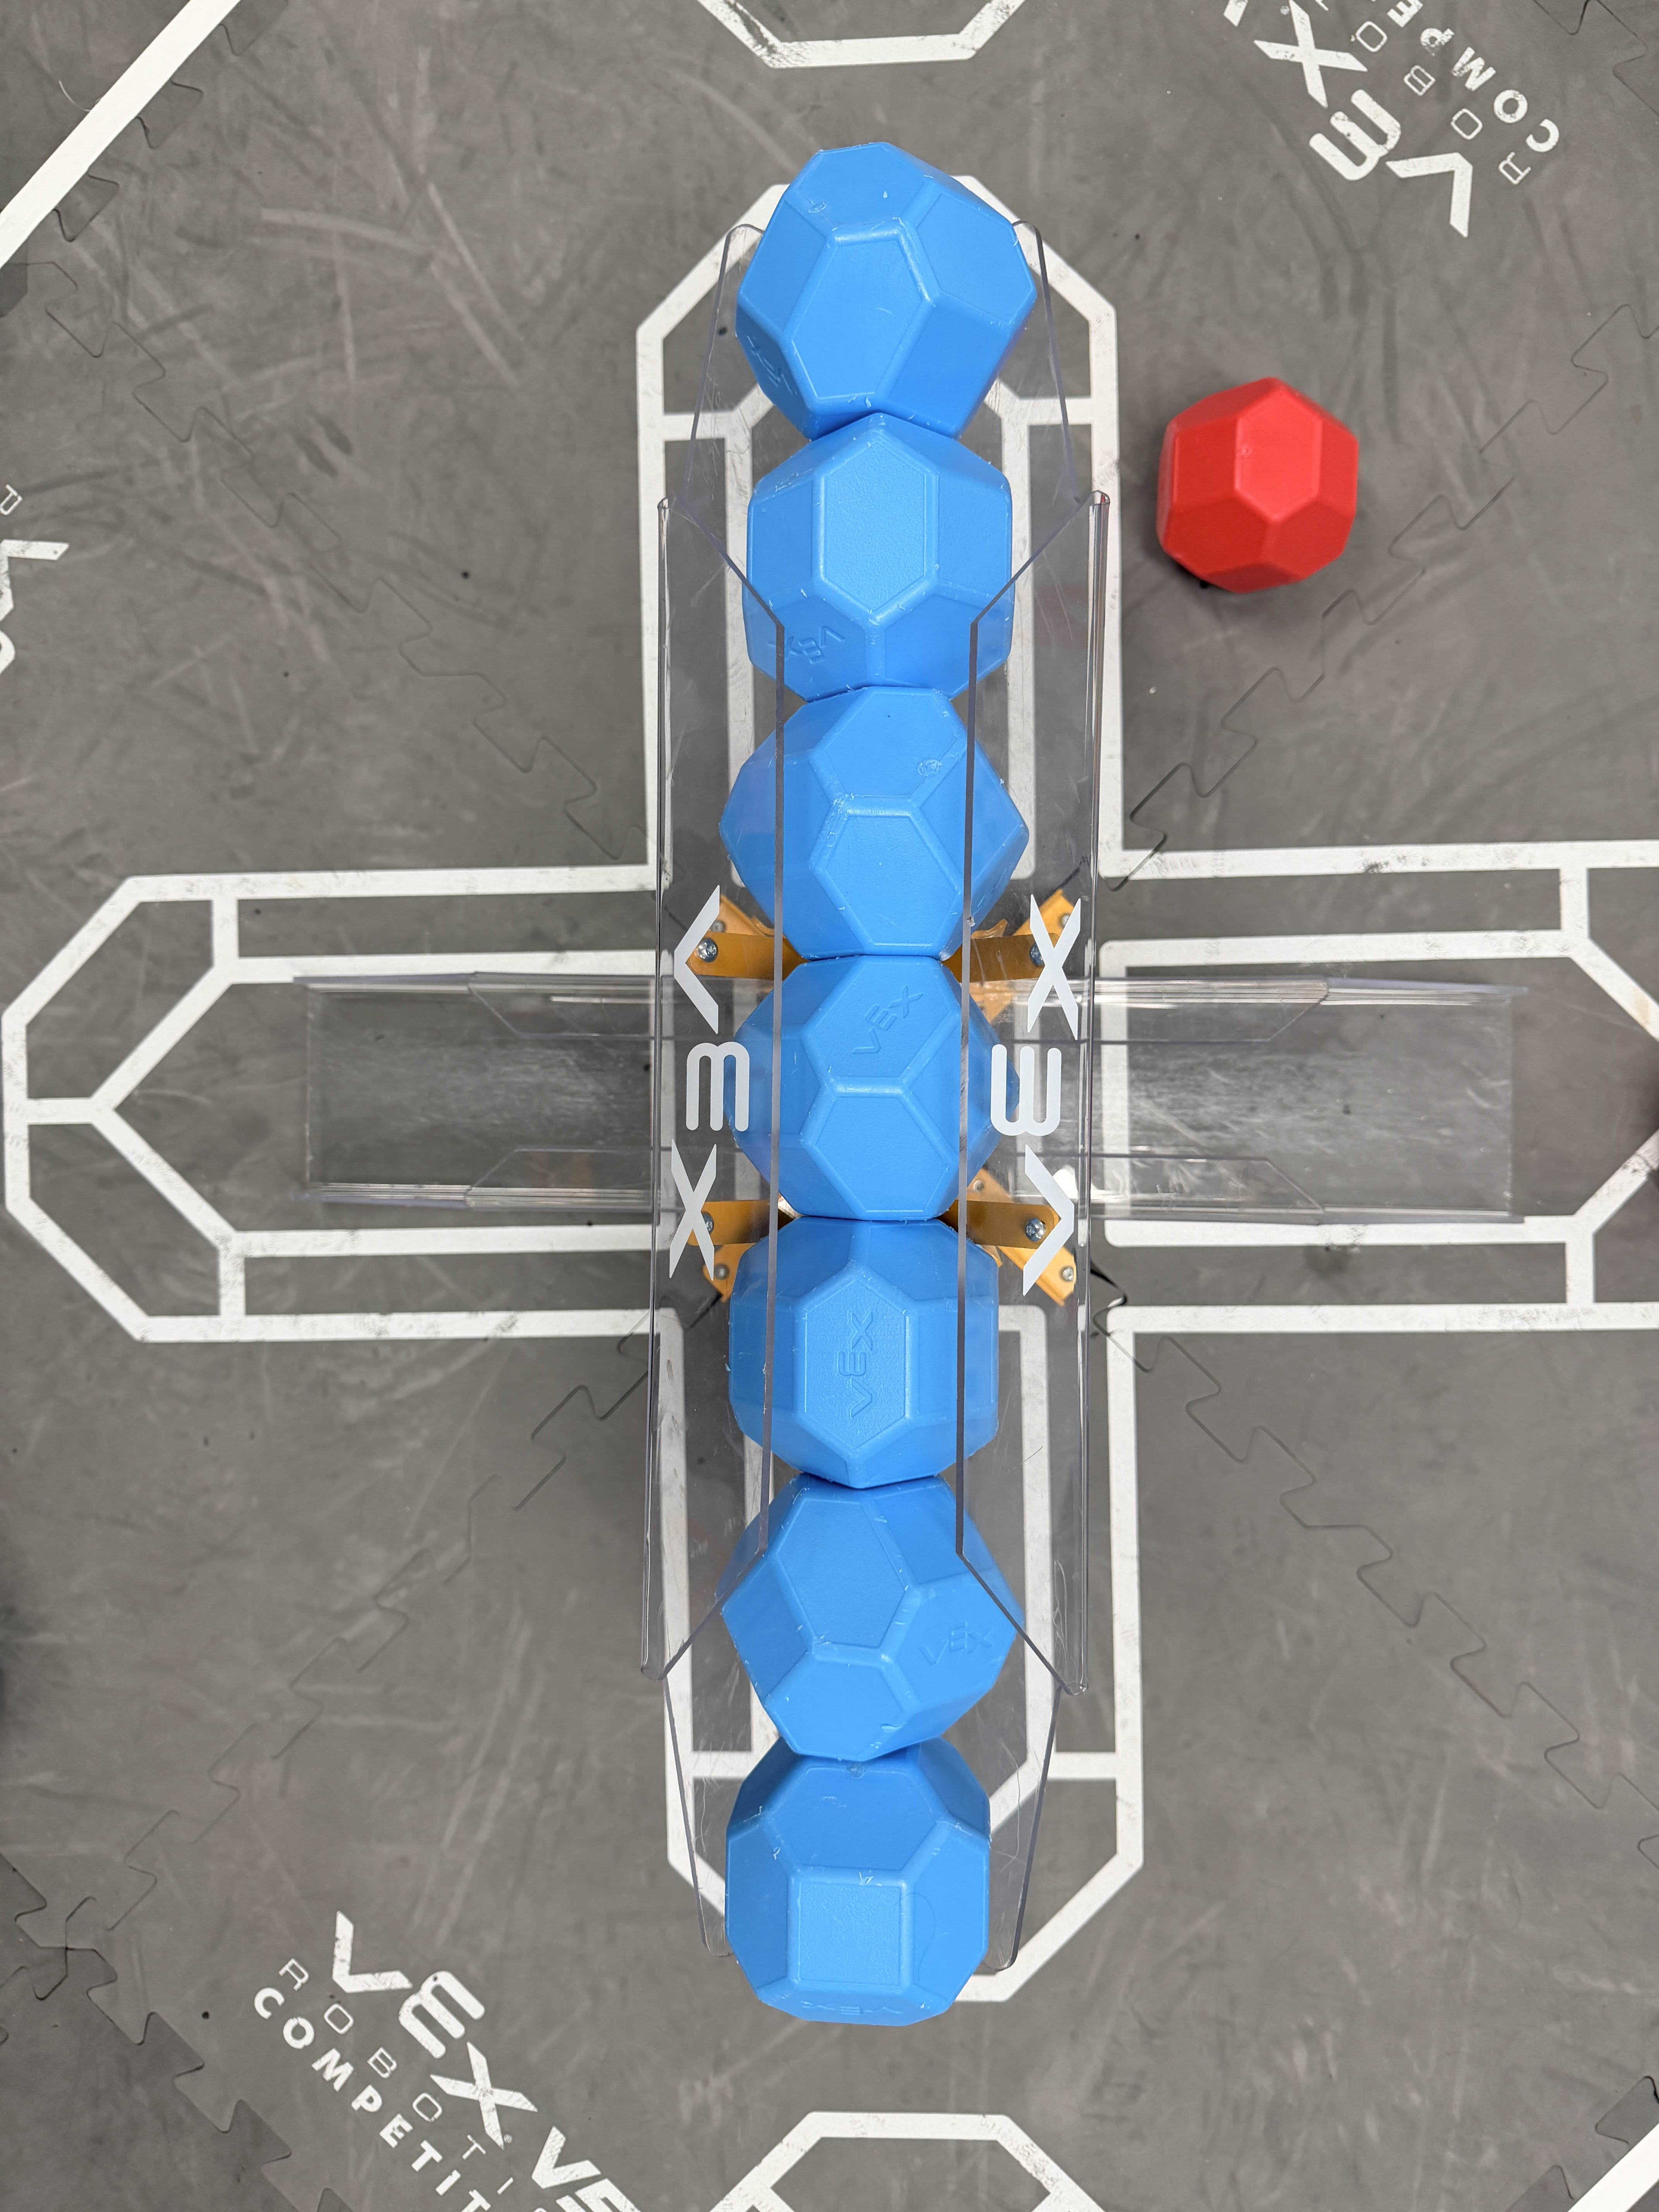
\includegraphics[width=0.95\linewidth, height=6.5cm]{images/Field and Field Elements/Max Middle_Goal.jpg}}
        \caption{Center Goal Max Capacity}
        \label{fig:Center_goal_max}
    \end{subfigure}
    
    \caption{Long Goal Capacity Analysis}
    \label{fig:long_goal_compare}
\end{figure}
    \end{itemize}
    \item Park Zones 
        \begin{itemize}
            \item These are located in the center of the outer walls where the driver station is located. 
             \begin{figure} [H]
    \centering
    \includegraphics[width=0.5\linewidth]{images/Field and Field Elements/ParkZone.png} 
    \caption{Red alliance Park Zone}
    \label{fig:Park_Zone}
\end{figure}
        \end{itemize}
        
     \item  Match Loaders
        \begin{itemize}
            \item For a total of 4 located at each end of the long goal on the alliance driver station wall. These Loaders hold a total of 6 balls; 3 red and 3 blue. 
            \begin{figure}[H]
    \centering
    % --- Image 1 (Left) ---
    \begin{subfigure}[b]{0.31\textwidth}
        \centering
        % 0.95 width to fit in border, 4.5cm height for uniformity
        \fbox{\includegraphics[width=0.95\linewidth, height=4.5cm]{images/Field and Field Elements/Loader.png}}
        \caption{Empty Match Loader}
        \label{fig:loader_empty}
    \end{subfigure}
    \hfill % Spacer 1
    % --- Image 2 (Middle) ---
    \begin{subfigure}[b]{0.31\textwidth}
        \centering
        \fbox{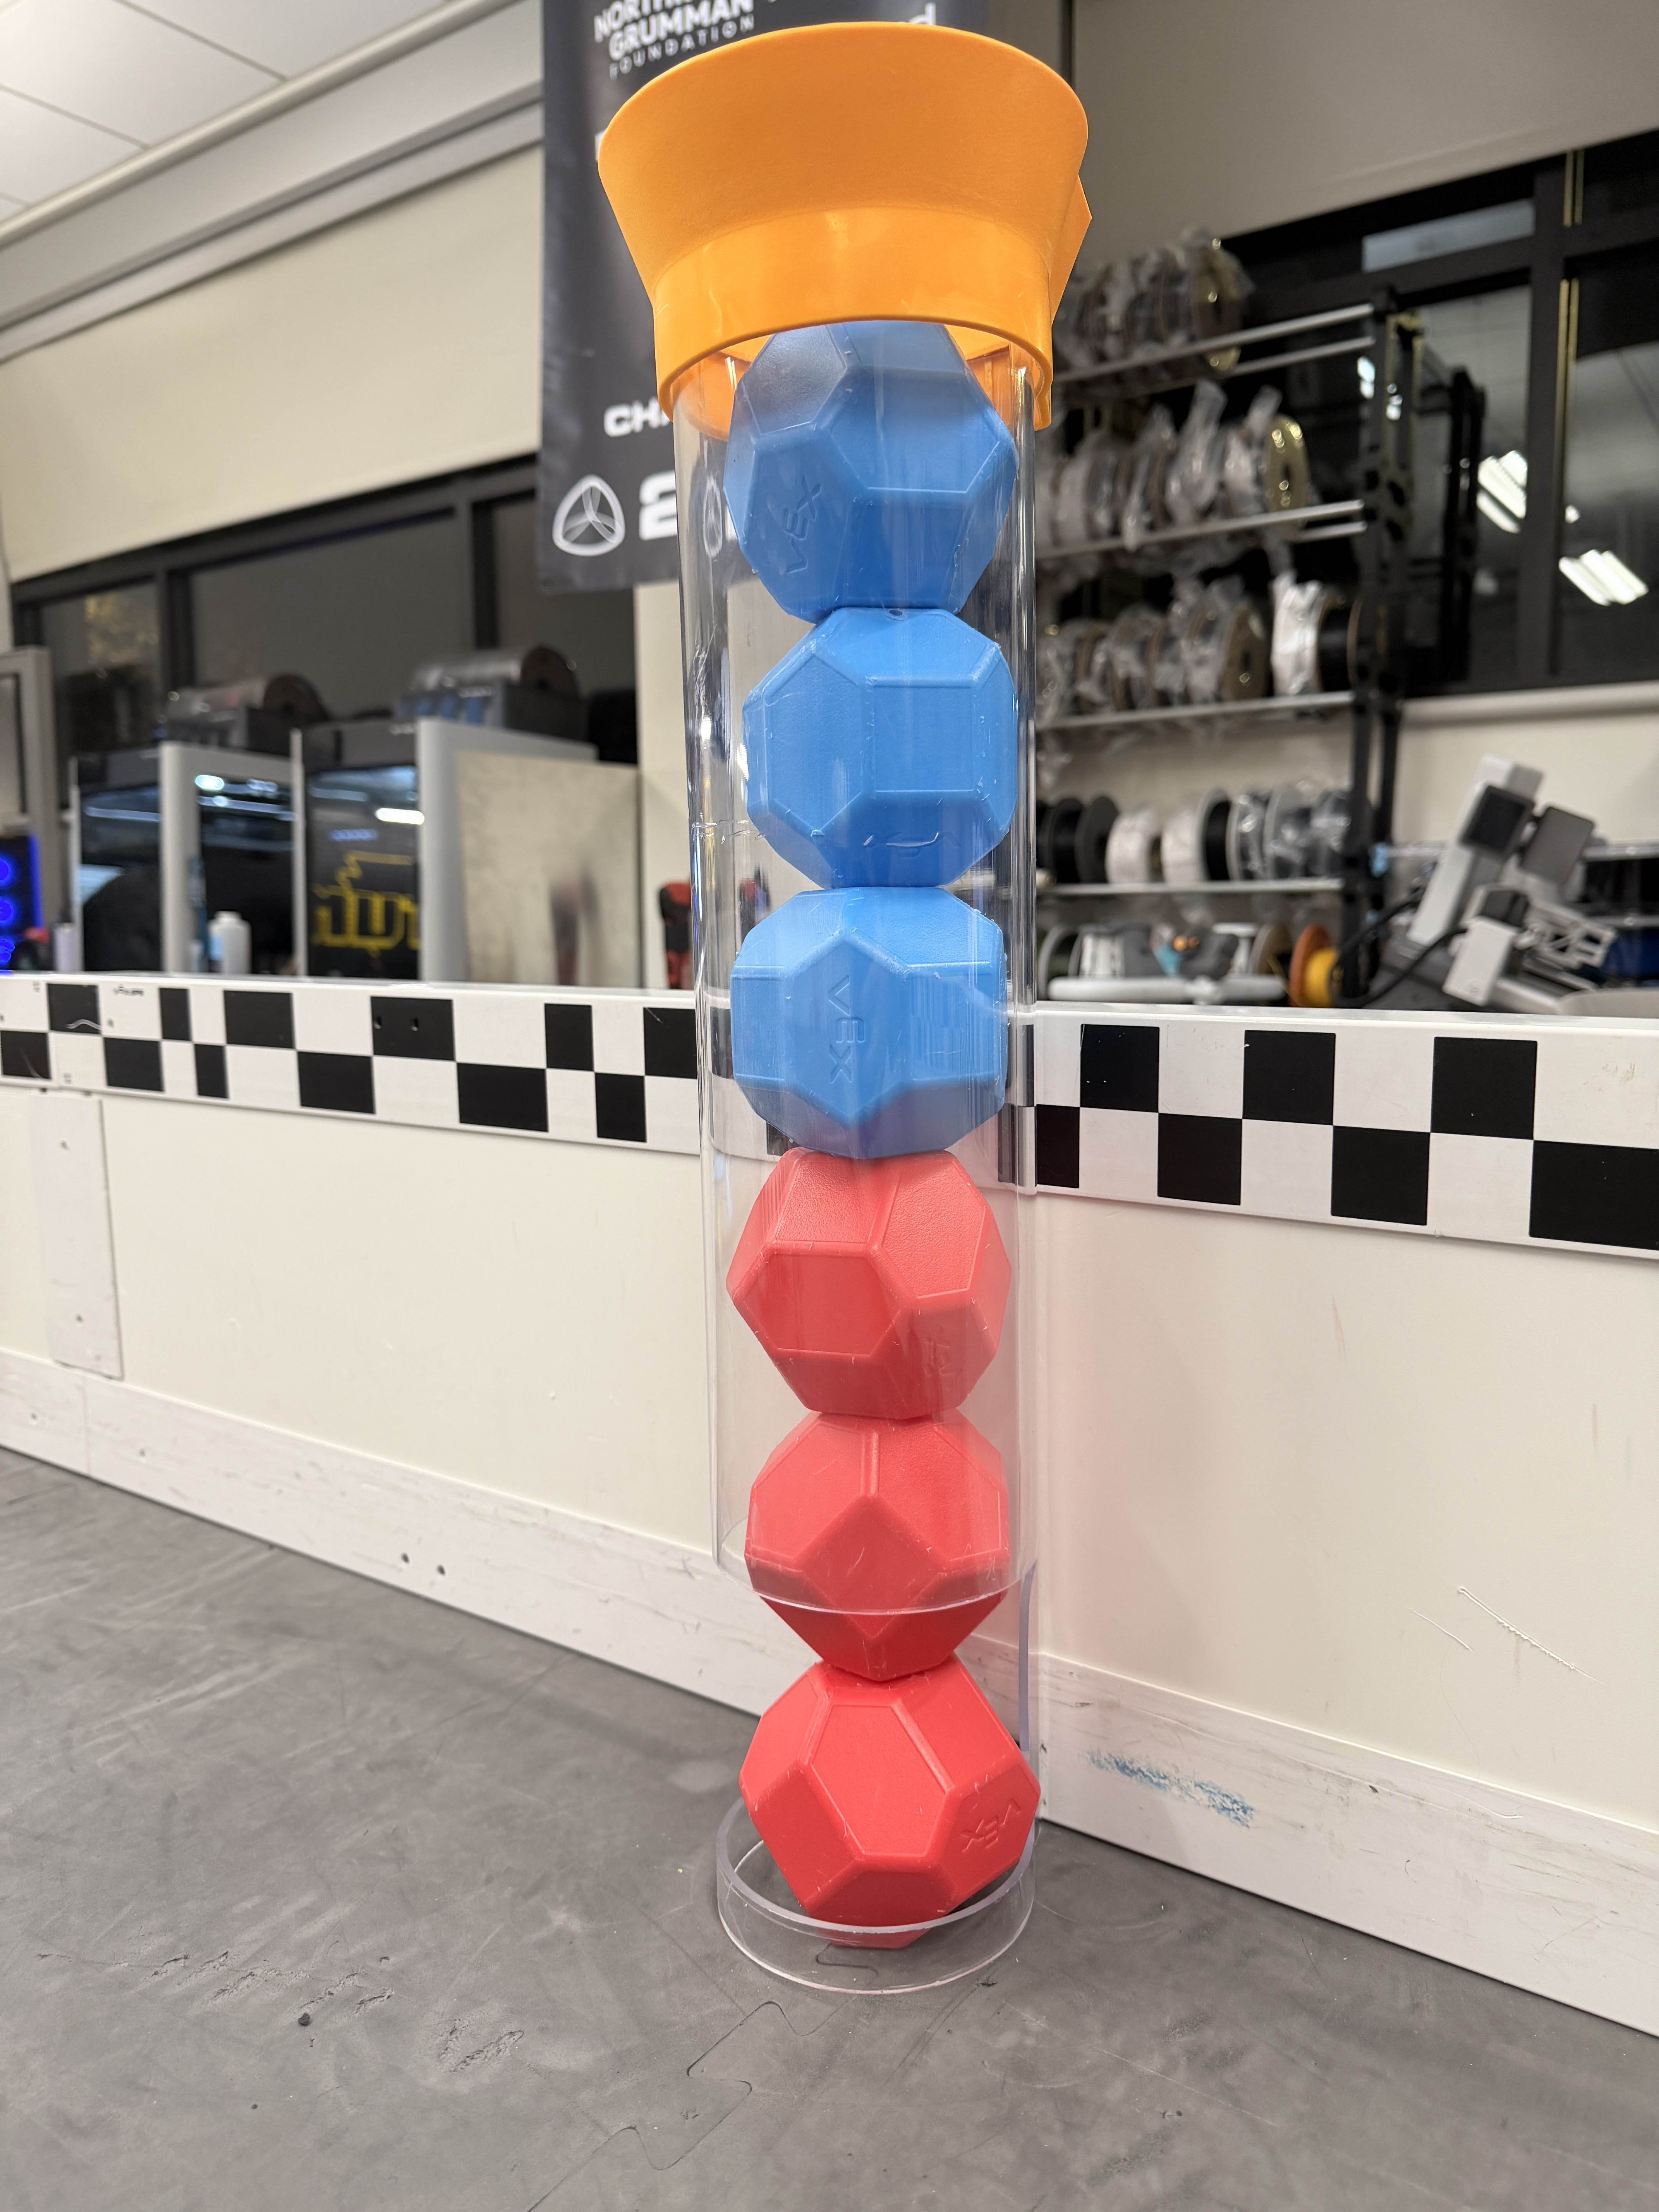
\includegraphics[width=0.95\linewidth, height=4.5cm]{images/Field and Field Elements/Red Alliance Loader.jpg}}
        \caption{Red Alliance Loader}
        \label{fig:loader_red}
    \end{subfigure}
    \hfill % Spacer 2
    % --- Image 3 (Right) ---
    \begin{subfigure}[b]{0.31\textwidth}
        \centering
        \fbox{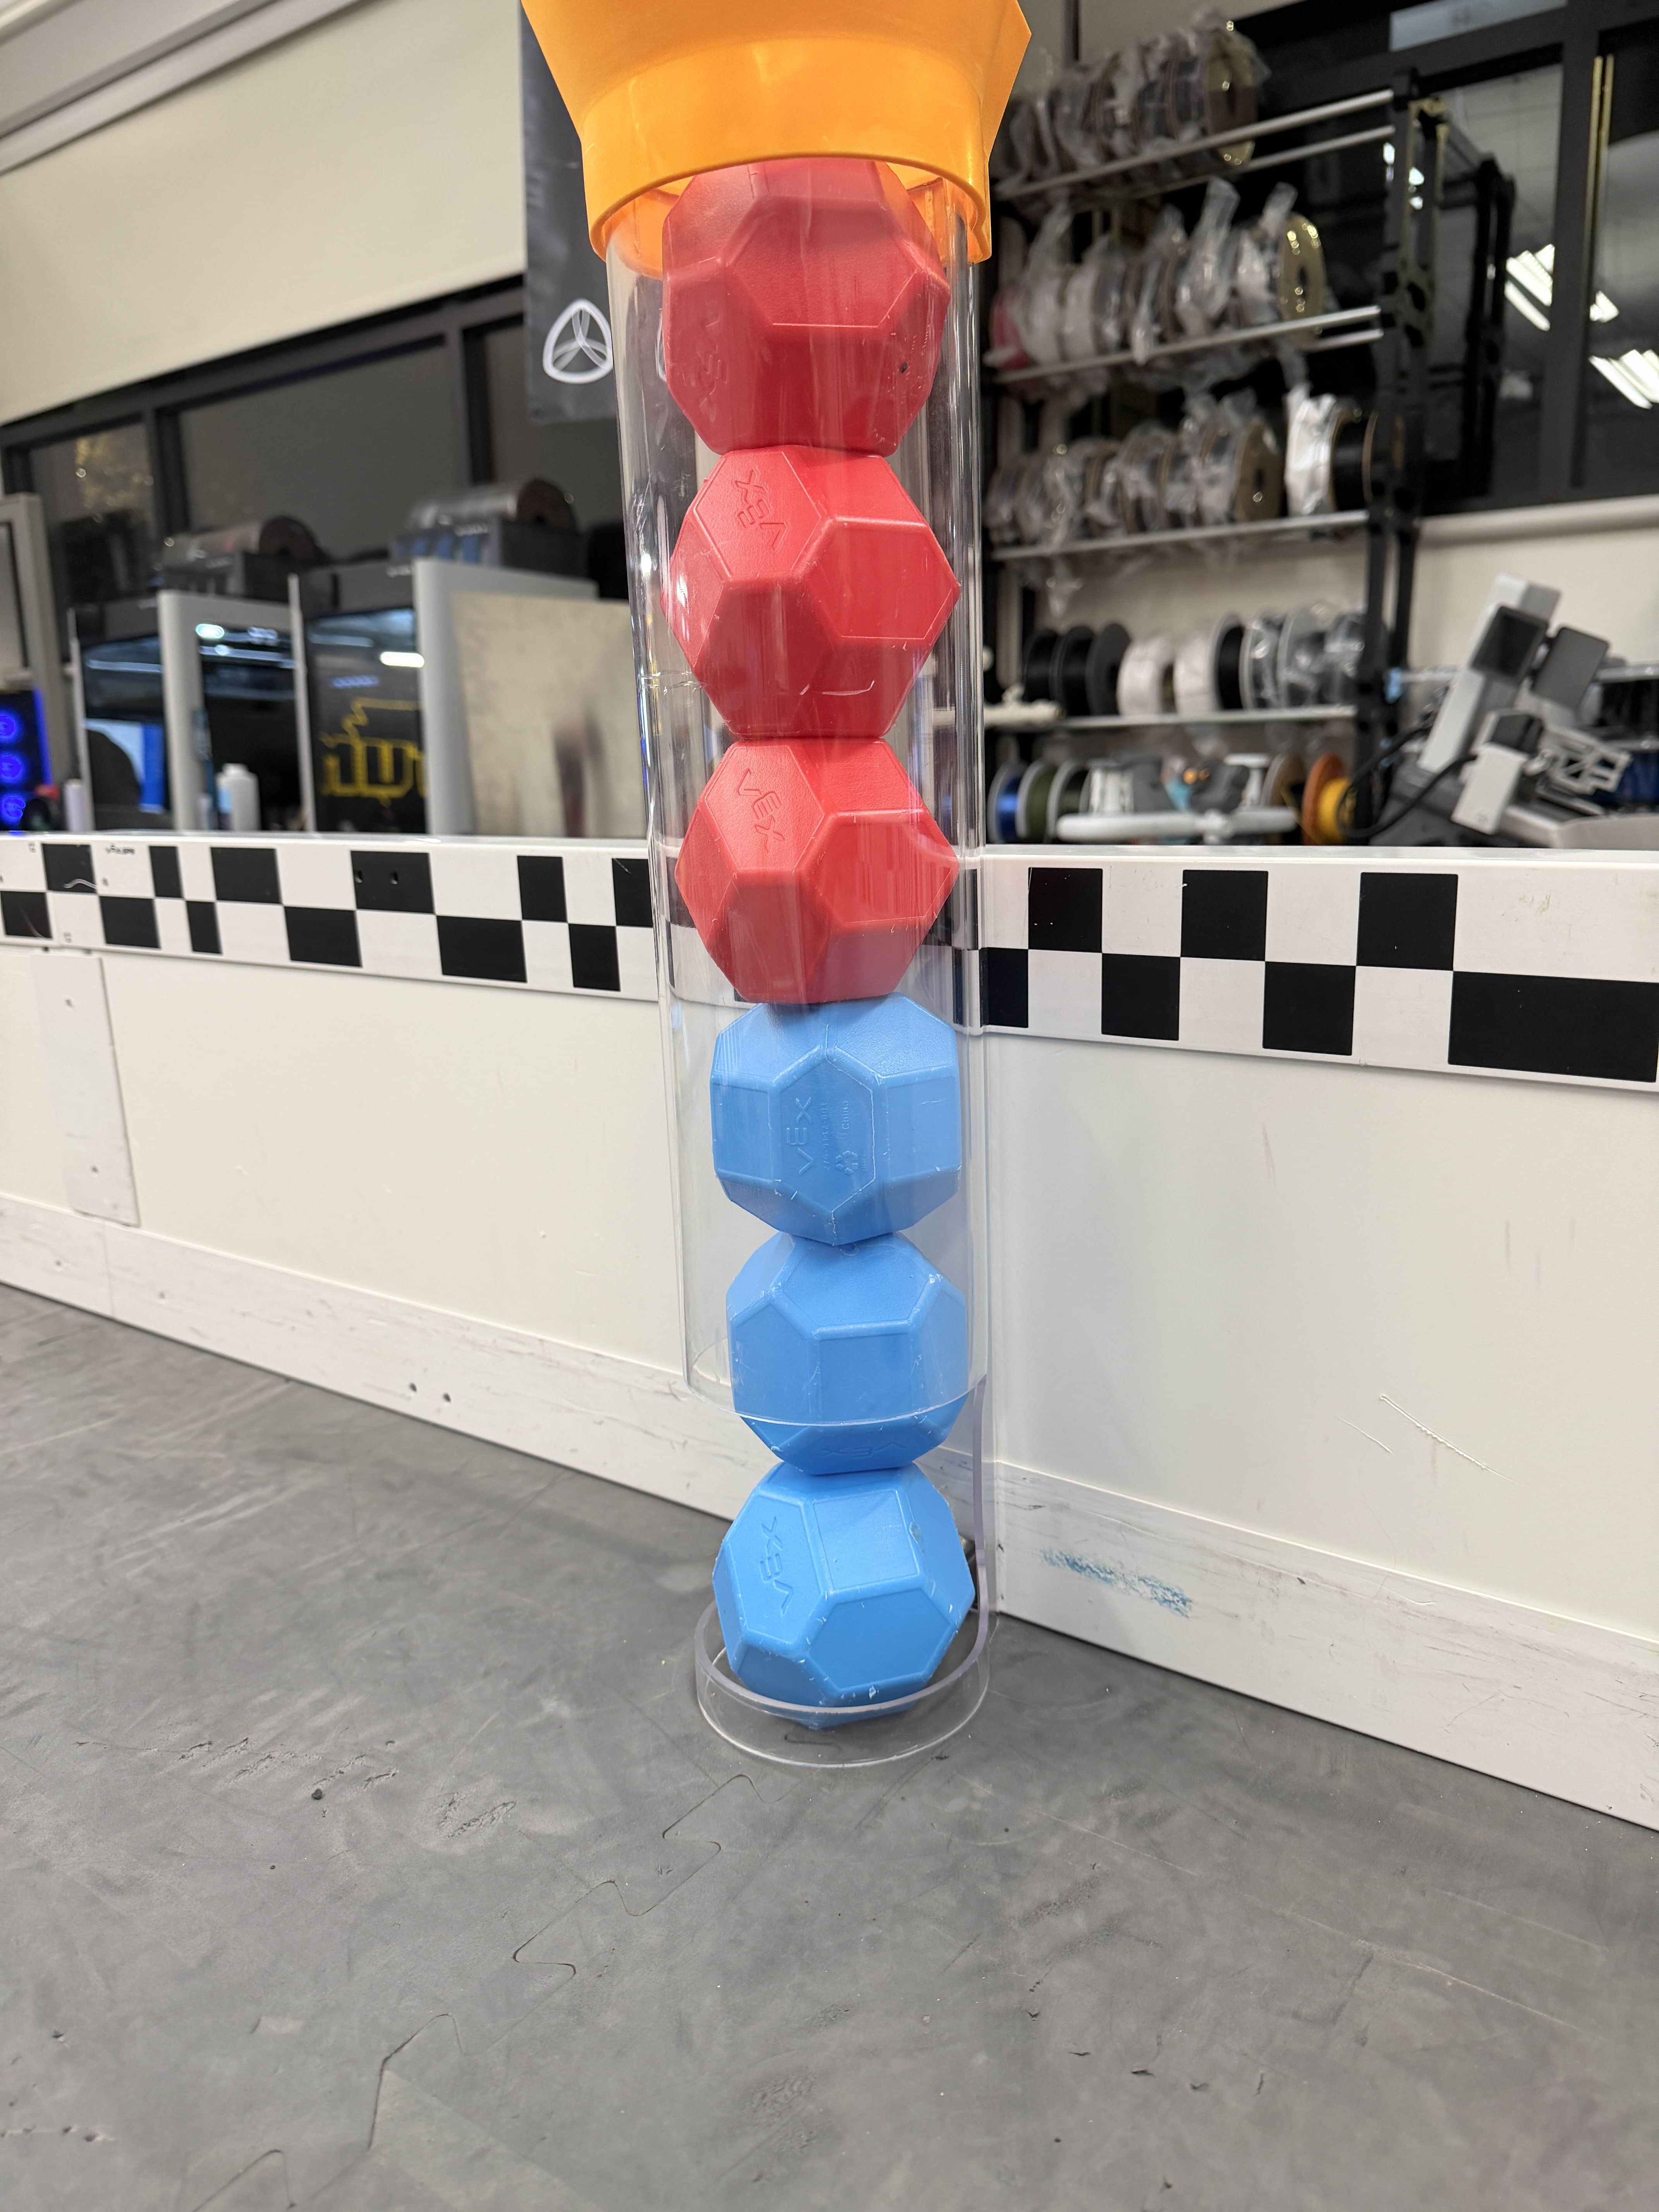
\includegraphics[width=0.95\linewidth, height=4.5cm]{images/Field and Field Elements/Blue Alliance Loader.jpg}}
        \caption{Blue Alliance Loader}
        \label{fig:loader_blue}
    \end{subfigure}
    \caption{Match Loader Configuration}
    \label{fig:loader_comparison}
\end{figure}
        \end{itemize}
    \end{itemize}
    
    \subsection{Game objects Rule analysis}
    Now that we have a outline of what will always be on the fields lets analysis rules that cover those said elements. 

    \begin{itemize}
    \item Blocks
    \begin{itemize}
        \item Infinite Possession
        \begin{itemize}
            \item  Compared to other seasons such as high stakes and over under which had a possession limit of 2 of the scoring elements, pushback removes this constraint and fundamentally shifts designs from a cycling design where you grab and score as fast as possible to a hoarding design. This means that the robot must have a feature such as a hopper or magazine capable of storing and scoring multiple blocks. 
        \end{itemize}
        \item Score Status (SC2)
        \begin{itemize}
            \item A block is considered scored if it meets the following criteria
            \begin{itemize}
                \item The block must be in contact with the edge faces of the inner surfaces of the goal. 
                \item The block can not contact a robot of the same color. 
                \item the block is not in contact with the floor. 
            \end{itemize}
            \item Although this rule seems straight forward it influences the design subtlety by ensuring that the scoring mechanism must have enough torque to score into the goal.
        \end{itemize}
        \item Point value 
        \begin{itemize}
            \item Each block scored is worth a total of 3 points. 
        \end{itemize}
    \end{itemize}
    \item Long goals
    \begin{itemize}
        \item Long goal Control (SC3)
        \begin{itemize}
            \item In order for a alliance to be in control of a long goal, a block must be fully contained within the control zone. It also must count as scored in the goal in order to be in control. 
        \end{itemize}
        \item Long Goal Point Value
        \begin{itemize}
            \item Control of a long zone is a additional 10 points to that alliances score. 
        \end{itemize}
    \end{itemize}
    \item Center Goals
    \begin{itemize}
        \item Center Goal Control (SC3)
        \begin{itemize}
            \item following part b. of SC3 the only requirement for the center goals is that the blocks must be considered scored and be the majority of the color within the goals. 
        \end{itemize}
        \item Center Goal Point Value 
        \begin{itemize}
            \item The control bonus for the upper goal is worth 8 points, while the lower goal control bonus is worth 6 points. 
        \end{itemize}
    \end{itemize}
    \item Park Zone
    \begin{itemize}
        \item Parking Criteria (SC4)
        \begin{itemize}
            \item There are three requirements in order for a robot to be considered parked; The robot is not contacting the floor outside fo the alliances colored parkzone, The robot is not contacting any other field element other then those considered the parkzone and inside of the barrier, and is at least partially within the vertical projection of the parkzone. 
        \end{itemize}
        \item Parking Point Values
        \begin{itemize}
            \item A singular parked robot is only worth 8 points. However, 2 parked robots increases the overall points to 30 points. That is almost double the points. 
        \end{itemize}
    \end{itemize}
    \item Match Loaders
    \begin{itemize}
        \item Match Loader Starting Blocks
        \begin{itemize}
            \item Each match loader begins with 3 red and 3 blue blocks inside of it for a total of 6 blocks. However, the orientation of said blocks depends on if the team is on the red or blue side. On the red alliance the match loads start with three red on the bottom three blue on top. The inverse is true for the blue alliance. 
        \end{itemize}
         \item Match Load introduction (SG9)
         \begin{itemize}
             \item VURC teams are allowed introduce balls during autonomous and driver control periods. 
             \item A match load can not contact a robot prior to being placed in loader, may only be removed by a robot through the bottom of the loader, and can only be introduced if there are no blocks partially or entirely within the orange portion of the loader. 
         \end{itemize}
    \end{itemize}
    \end{itemize}
    
     \subsection{Design and Strategy Considerations.}
     After going through the standard field layout, we have a general idea for what we need to design for and consider for strategies 
    \newline
    
     \subsection{Design Requirements}
        Lets consider that a long goal is considered as the max amount of blocks we need to score. That would implies that our robot would need to store and score 15 blocks in succession. However, this assumption is unrealistic and doesn't take in many factors so lets plan for the worse case scenario. 
     \newline   
        \indent In the worse case scenario we still need to score at least a theoretical "51\%." Meaning that if a long goal holds 15 blocks our robot needs to be able to score at least 8 balls in succession. With this requirement we also cover our need "51\%" for the center goals since they require 4 blocks at a minimum. 
        \newline
        \indent The parkzone adds in a unique challenge for this year. While one parked robot only adds 8 points, two parked robots gives a overall point value of 30 points effectively doubling the points you would receive from two individually parked bots. 
        \newline
        \indent Match loaders introduce a unique problem. Although you are able to remove the blocks of you alliance colors you still need to remove the opponents color in order to match load the remaining blocks outside of the field. There are two methods for doing this one is in-taking said blocks moving back turning and out-taking to remove those blocks. However, this takes precious time and effort that could be otherwise used in order to establish a winning position. The second method is developing a "Color Sort" in order to automatically remove blocks out of the system without having to take other actions. A color sort is the best option due to it taking less actions and saving time that can be used elsewhere.
        
    \subsection{Strategies}
    There is a possible 44 blocks to be scored, 15 in each long long and 7 in the centers goals. 

\begin{table}[h!]
    \centering
    \caption{\textbf{Pushback Scoring Matrix}}
    \label{tab:scoring_matrix}
    \begin{tabular}{lccc}
        \toprule
        \textbf{Scoring Object} & \textbf{Block Value} & \textbf{Block Amount} & \textbf{Control Bonus} \\
        \midrule
        Long Goal 1 & 3 & 15 & 10 (\checkmark) \\
        Long Goal 2 & 3 & 15 & 10 (\checkmark) \\
        Center Goal (Upper) & 3 & 7 & 8 (\checkmark) \\
        Center Goal (Lower) & 3 & 7 & 6 (\checkmark) \\
        \bottomrule
    \end{tabular}
\end{table}

If we include a double parked alliance for a total of 30 points, and the autonomous bonus. The maximum points that a alliance can have is 206 points. if we take in account the worse case scenario that we need to score a minimum of 51\% of the total points the total comes to approximately 106 points. 
\newline 
\indent Breaking down the point value we can start to see what our design should be able to do. For example, out of a 106 points a double parked alliance is worth 30 points which accounts for 28\% of the minimum points this immediately raises concern that our robots should be able to double park as that accounts for more then a quarter of the points we need. 
\newline
\indent That leaves 76 points that need to be scored via control bonus and blocks. If we assume that we score the minimum amount of balls in order to establish control of both long goals. 

\begin{table}[h!]
    \centering
    \caption{\textbf{Minimum Long Goal Scoring}}
    \label{tab:scoring_matrix}
    \begin{tabular}{lccc}
        \toprule
        \textbf{Scoring Object} & \textbf{Block Value} & \textbf{Block Amount} & \textbf{Control Bonus} \\
        \midrule
        Long Goal 1 & 3 & 8 & 10 (\checkmark) \\
        Long Goal 2 & 3 & 8 & 10 (\checkmark) \\
        \bottomrule
    \end{tabular}
\end{table}

That gives us a total of 68 of the 76 remaining points. This means that we only need to score 3 more blocks in any of the goals to establish a winning position during the match. 
\newline

\subsection{Review}
    Now we have some constraints that were otherwise not listed or known
    \subsubsection{Constraints}
    \begin{itemize}
        \item Our robots must have a capacity of at least 8 blocks in order to establish control over the goals. 
        \item Both bots must be able to work together in order to establish a double park. 
        \item Working together both bots must be able to score at least 51\% of the total points in order to establish a winning position. 
    \end{itemize}

   \section{VURC Format Modifications}
Now that we have looked at the constants on the field its time to look at the differences between V5RC and VURC. As a VEX U team, we compete under the VURC Section 6 rulset:

\subsection{Rule Modifications: Robot (Appendix C)}
VURC Robot rules transform the competition from a "kit-based" challenge to an "open-class" engineering challenge. The following modifications allow Team ATUM to utilize industrial manufacturing techniques and custom electronics.

\subsubsection{1. Chassis \& Configuration (VUR1)}
\begin{itemize}
    \item \textbf{Rule:} A VURC Alliance consists of two robots:
    \begin{itemize}
        \item One robot must fit within $24'' \times 24'' \times 24''$.
        \item One robot must fit within $15'' \times 15'' \times 15''$.
    \end{itemize}
    \item \textbf{Strategic Implication:} While permitted to build a large robot, Team ATUM has elected to field \textbf{two 15'' robots}. We are voluntarily sacrificing the volume of the 24'' constraint to gain the advantage of identical mechanical architecture (efficiency) and lower field congestion (mobility).
\end{itemize}

\subsubsection{2. Materials \& Fabrication (VUR3 - VUR7)}
\begin{itemize}
    \item \textbf{Rule:} Teams may fabricate parts from raw stock (aluminum, steel, plastic) and use additive manufacturing (3D printing).
    \item \textbf{Strategic Implication (Drivetrain):} We will utilize this rule to CNC machine \textbf{custom 6061 Aluminum side plates} along with \textbf{3D printed parts}. This is the only way to package an 10-motor vertical stack within the 15'' limit; standard VEX c-channels are too bulky.
    \item \textbf{Strategic Implication (Intake):} We will use 3D printed  geometries to create "perfect fit" intake pathways for the Blocks, rather than relying on flat VEX gussets.
    \item \textbf{Safety Note (VUR6):} We will strictly avoid shattering plastics like Acrylic/Plexiglass, opting instead for Polycarbonate (Lexan) to prevent field debris hazards.
\end{itemize}

\subsubsection{3. Motors \& Power (VUR11)}
\begin{itemize}
    \item \textbf{Rule:} There is \textbf{no limit} on the number of V5 Smart Motors (11W or 5.5W).
    \item \textbf{Strategic Implication:} In V5RC (High School), an 8-motor drive leaves no motors for mechanisms. In VURC, we can run an \textbf{10-Motor Drivetrain (110W)} for maximum torque while still allocating sufficient motors for high-speed Intakes and Conveyors. Power management, not motor quantity, becomes the limiting factor.
\end{itemize}

\subsubsection{4. Commercial Components (VUR8, VUR9, VUR15)}
\begin{itemize}
    \item \textbf{Rule:} Teams may use commercially available springs, fasteners, and bearings.
    \item \textbf{Strategic Implication:}
    \begin{itemize}
        \item \textbf{Bearings (VUR15):} We will replace standard VEX plastic bearings with high-tolerance steel ball bearings to minimize friction in the high-load drivetrain.
        \item \textbf{Fasteners (VUR9):} We will use high-strength steel screws and thread-locker (Loctite) to ensure reliability under heavy defense.
    \end{itemize}
\end{itemize}

\subsubsection{5. Electronics \& Sensors (VUR10, VUR12, VUR13)}
\begin{itemize}
    \item \textbf{Rule:} Teams may use custom sensors (LIDAR, cameras) and external processors (Raspberry Pi, Jetson), provided they do not directly power motors.
    \item \textbf{Restriction (VUR13):} Pre-made "Electromechanical Assemblies" (like commercial odometry pods) are banned.
    \item \textbf{Strategic Implication:} We will design and print \textbf{custom odometry pods} to house commercial rotary encoders. This gives us the precision of industrial sensors while remaining compliant with the "no pre-made assemblies" rule.
\end{itemize}

\subsubsection{6. Pneumatics (VUR14)}
\begin{itemize}
    \item \textbf{Rule:} Teams may use an unlimited number of pneumatic reservoirs and cylinders, charged to 100 PSI.
    \item \textbf{Strategic Implication:} The 100 PSI limit combined with unlimited volume allows us to use pneumatics for high-force applications, such as a localized "Plow" or "Descoring" mechanism, without running out of air.
\end{itemize}

\subsection{Rule Modifications: Game (Appendix C)}
VURC Appendix C introduces specific gameplay modifications that differ from the V5RC manual. These rules (VUG> through VUG7) dictate how we must play the match and influence our autonomous strategy.

\begin{itemize}
    \item \textbf{VUG1 Robot Placement Strategy:}
    \\ The Red Alliance places one robot, then the Blue Alliance places both robots, and finally the Red Alliance places their second robot.
    \\ \textit{Strategic Implication:} This gives the Red Alliance a counter-deployment advantage. As a "Twin 15" team, our robots are identical, which hides our strategy slightly, but we must have versatile autonomous routines that function regardless of whether we are placed first or last.

    \item \textbf{VUG2 Expansion Limits:}
    \\ The designated 24'' Robot may expand to the full $24'' \times 24'' \times 24''$ volume at any time.
    \\ \textit{Strategic Implication:} While Team ATUM is running two 15'' robots we can have a "Expansion" on one of the bots in order to start it further from its required starting position as long as it still fits the 24" starting volume. 

    \item \textbf{VUG3 Continuous Loading:}
    \\ Match Load Blocks may be introduced during \textbf{both} the Autonomous and Driver Controlled periods.
    \\ \textit{Strategic Implication:} This validates our high-capacity intake design. As we are able to safely secure 8 blocks during the autonomous period without taking risk in the neutral zone. 

    \item \textbf{VUG4 Autonomous Win Point (AWP) Criteria:}
    \\ The AWP in VURC is significantly more difficult than V5RC. To earn the point, we must complete \textbf{ALL} of the following:
    \begin{enumerate}
        \item Score at least 12 Blocks.
        \item Score in at least 3 different Goals.
        \item Clear all 6 Match Load blocks from the loader.
        \item Park at least one robot.
    \end{enumerate}
    \textit{Strategic Implication:} This checklist is impossible for a single robot to complete in 30-45 seconds. This implies that we must split the task in between both bots in order to met the requirements in the time constraint. 

    \item \textbf{VUG5 \& VUG6 Neutral Zone Engagement:}
    \\ Interaction within the Neutral Zone is "At Your Own Risk." Robots entering the zone must expect contact.
    \\ \textit{Strategic Implication:} The center of the field will be a combat zone during Autonomous. We cannot build fragile intake deployments. Our "Twin 15" robots must have robust, shock-absorbing intake guards to survive high-speed collisions with opponents rushing for the same Neutral Zone blocks.
\end{itemize}

